\documentclass[11pt,a4paper]{ivoa}
\input tthdefs

\SVN$Rev$
\SVN$Date$
\SVN$URL$


\iftth
\message{Define parameters env for tth (ask markus)}
\ddt
\else
\newenvironment{parameters}%
% this is *only* for use within a description environment
  {\hfil % let definition label stand on a line of its own.
    \begin{list}{$\bullet$}{\topsep=0pt\partopsep=0pt\parsep=0pt}
    }%
  {\end{list}}
\fi

\title{Catalogue of ADQL User Defined Functions}

% see ivoatexDoc for what group names to use here
\ivoagroup{DAL}

\author{Jon Juaristi Campillo}
\author[https://wiki.ivoa.net/twiki/bin/view/IVOA/MarkusDemleitner]{Markus Demleitner}


\editor{Jon Juaristi Campillo}

% \previousversion[????URL????]{????Funny Label????}
\previousversion{This is the first public release}
       

\begin{document}
\begin{abstract}
The endorsed content of this note documents the consensus on ADQL user
defined functions (UDFs) with an \verb|ivo_| prefix, either by
referencing recommendations that defined the function, or by defining
functions in place.  A non-normative appendix lists UDFs declared by
registered TAP services.
\end{abstract}


\section*{Conformance-related definitions}

The words ``MUST'', ``SHALL'', ``SHOULD'', ``MAY'', ``RECOMMENDED'', and
``OPTIONAL'' (in upper or lower case) used in this document are to be
interpreted as described in IETF standard RFC2119 \citep{std:RFC2119}.

The \emph{Virtual Observatory (VO)} is a
general term for a collection of federated resources that can be used
to conduct astronomical research, education, and outreach.
The \href{http://www.ivoa.net}{International
Virtual Observatory Alliance (IVOA)} is a global
collaboration of separately funded projects to develop standards and
infrastructure that enable VO applications.


\section{Introduction}

The Astronomical Data Query Language ADQL \citep{2008ivoa.spec.1030O}
has the notion of user defined fucntions (UDF).  These provide a
light-weight extension mechanism for operators of TAP services.  
For instance, \citet{2016arXiv161109190T} shows how they enable the
construction of HEALPix maps although ADQL~2.0 itself entirely lacks
facilities to deal with them.

In order to provide a reliable core set of such functions that, if
present, have a constant meaning across multiple services, ADQL 2.1
(still under review at the time of writing) will stipulate that user
defined functions with names starting with \verb|ivo_| are to be used
and defined interoperably, i.e., there should be an IVOA-wide consensus
on their names and semantics. 

This note documents this consensus where it has been reached within
other standards, and reviews of this document are the preferred way to
introduce new \verb|ivo_| UDFs.

Note that no function given here is required to be present in a generic
TAP service (though other standards may pose such requirements;
\verb|ivo_hashlist_has|, for instance, is, or will be, required by both
RegTAP and EPN-TAP).  However, if a service implements any UDF with a
name starting with \verb|ivo_|, its semantics must be as specified here.

Informationally, in each revision of this document, we also run an
all-VO survey of user defined functions in registered TAP services.  The
result of this survey is available as an appendix (which, by
construction, is non-normative).

%\subsection{Role within the VO Architecture}

%\begin{figure}
%\centering

%% As of ivoatex 1.2, the architecture diagram is generated by ivoatex in
% SVG; copy ivoatex/archdiag-full.xml to archdiag.xml and throw out
% all lines not relevant to your standard.
% Notes don't generally need this.  If you don't copy archdiag.xml,
% you must remove archdiag.svg from FIGURES in the Makefile.

%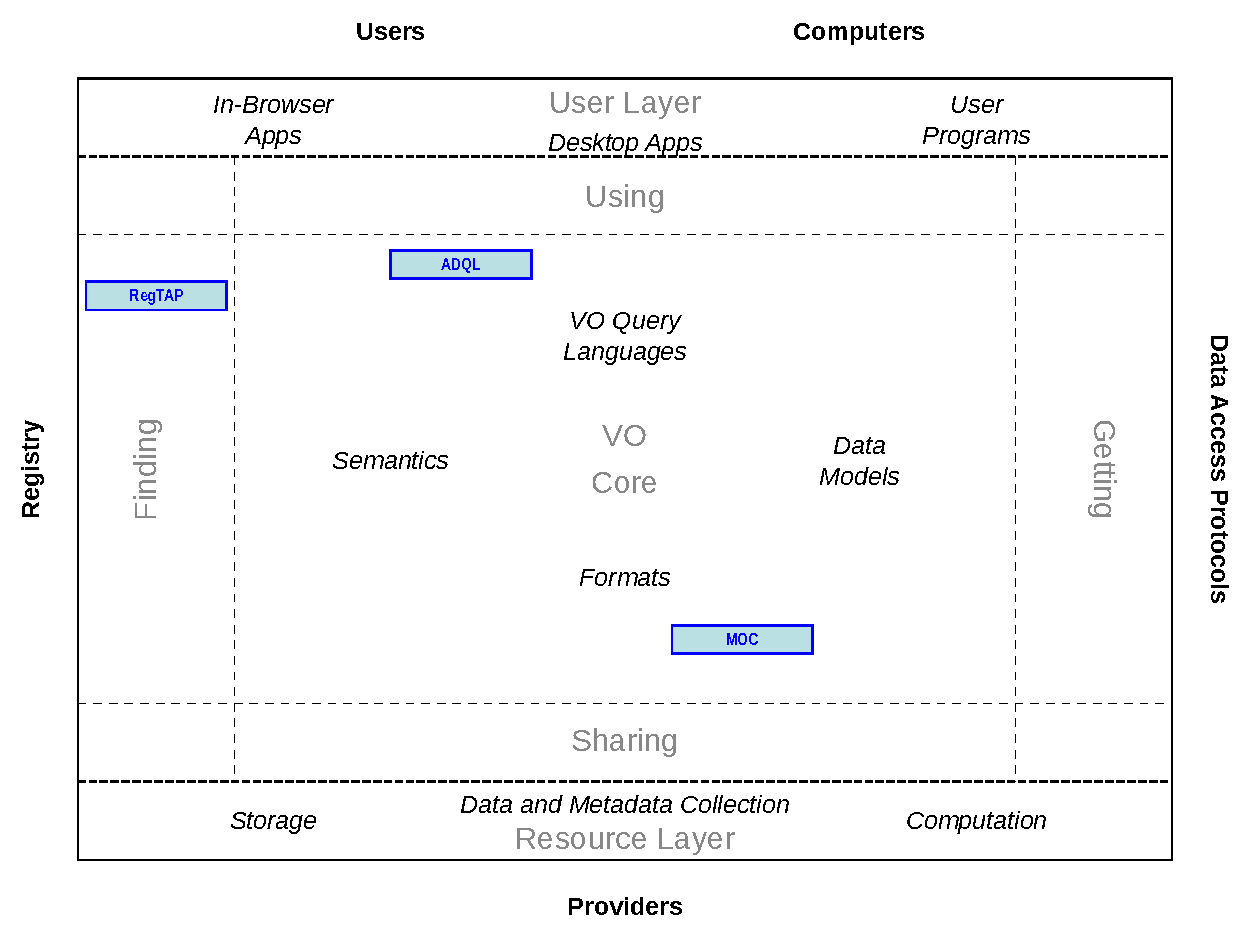
\includegraphics[width=0.9\textwidth]{role_diagram.pdf}
%\caption{Architecture diagram for this document}
%\label{fig:archdiag}
%\end{figure}

%Fig.~\ref{fig:archdiag} shows the role this document plays within the
%IVOA architecture \citep{note:VOARCH}.

%???? and so on, LaTeX as you know and love it. ????

\section{List of IVOA user defined functions}
\subsection{HEALPix-related}

In this section, order and npix are used as in the MOC recommendation
\citep{2014ivoa.spec.0602F}.

\subsubsection{\texttt{ivo\_healpix\_index(hpxOrder, ra, dec)}}

Returns the index (npix) of the Healpix cell containing the spherical
point given by right ascension \texttt{ra} and declination \texttt{dec}
at order \texttt{hpxOrder} in NESTED numbering.

\begin{description}
\item[Parameters]

\begin{parameters}
	\item hpxOrder (\texttt{INTEGER})
	\item ra (\texttt{DOUBLE})
	\item dec (\texttt{DOUBLE})
\end{parameters}

\item[Return type] \texttt{BIGINT}

\item[Source] This document.
\end{description}

\subsubsection{\texttt{ivo\_healpix\_index} with a spherical point}

Parameters:

\begin{itemize}
	\item hpxOrder (\texttt{INTEGER})
	\item point (\texttt{POINT})
\end{itemize}

Returns: \texttt{BIGINT}

Source: This document.

Returns the index (npix) of the HEALPix cell containing the spherical
point given by \texttt{point} at order \texttt{hpxOrder} in NESTED
numbering.


\subsubsection{ivo\_healpix\_center}

Parameters:

\begin{itemize}
	\item hpxOrder (\texttt{INTEGER})
	\item hpxIndex (\texttt{INTEGER})
\end{itemize}

Returns: \texttt{POINT}

Source: This document

Returns a \texttt{POINT} corresponding to the center of the HEALPix cell
with index (npix) \texttt{hpxIndex} at order \texttt{hpxOrder}.

\subsubsection{\texttt{ivo\_apply\_pm}}

Parameters:

\begin{itemize}
	\item ra (\texttt{DOUBLE})
	\item dec (\texttt{DOUBLE})
	\item pmra (\texttt{DOUBLE})
	\item pmdec (\texttt{DOUBLE})
	\item epochDist (\texttt{DOUBLE})
\end{itemize}

Returns: \texttt{POINT}.

Source: This document

Returns a \texttt{POINT} for the position an object at \texttt{ra},
\texttt{dec} will be at after \texttt{epochDist} Julian years if its proper
motion is \texttt{prma}, \texttt{pmdec}.  Positions must be in degrees,
proper motions are expected in degrees/year. The proper motions must be
given in the tangential plane (,,contain $cos(\delta)$'').

Note that this is an operation of spherical geometry, i.e., the function
would work as well with non-equatorial coordinates \emph{and} proper
motions.  However, you cannot, of course, mix galactic coordinates with
equatorial proper motions.


\subsection{Text related}

\subsubsection{ivo\_string\_agg}

Parameters:

\begin{itemize}
	\item expression (\texttt{TEXT})
	\item delimiter (\texttt{TEXT})
\end{itemize}

Returns: \texttt{TEXT}

Source: RegTAP \citep{2014ivoa.spec.1208D}

An aggregate function returning all values of \texttt{expression} 
concatenated with delimiter.

\subsubsection{ivo\_nocasematch}

Parameters:

\begin{itemize}
	\item value (\texttt{TEXT})
	\item pattern (\texttt{TEXT})
\end{itemize}

Returns: \texttt{INTEGER}

Source: RegTAP \citep{2014ivoa.spec.1208D}

Pattern is defined as for the SQL LIKE operator, but the match is
performed case-insensitively. This function in effect provides a
surrogate for the ILIKE SQL operator that is missing from ADQL. Returns
1 if pattern matches, 0 otherwise.

In ADQL 2.1 and later, use the ILIKE operator instead.

\subsubsection{ivo\_hasword}

Parameters:

\begin{itemize}
	\item haystack (\texttt{TEXT})
	\item needle (\texttt{TEXT})
\end{itemize}

Returns: \texttt{INTEGER}.

Source: RegTAP \citep{2014ivoa.spec.1208D}

Returns 1 if the string \texttt{needle} is contained (in some sense) in
the string \texttt{haystack}, 0 otherwise.  This is intended to support
somewhat ``Google-like'', soft string matches.

\subsubsection{ivo\_hashlist\_has}

Parameters:

\begin{itemize}
	\item hashlist (\texttt{TEXT})
	\item item (\texttt{TEXT})
\end{itemize}

Returns: \texttt{INTEGER}

Source: RegTAP \citep{2014ivoa.spec.1208D}

The \texttt{hashlist} argument is a list of words not containing the hash
sign (\#), concatenated by hash signs; the \texttt{item} argument is
a string not containing a hash sign. The function
returns 1 if, compared case-insensitively,
the second argument is in the list of words encoded in the first argument.
The behaviour in case the second argument contains a hash sign is
unspecified.

\subsection{Interval Arithmetic}

\subsubsection{ivo\_interval\_overlaps}

Parameters:

\begin{itemize}
	\item l1 (\texttt{NUMERIC})
	\item h1 (\texttt{NUMERIC})
	\item l2 (\texttt{NUMERIC})
	\item h2 (\texttt{NUMERIC})
\end{itemize}

Returns \texttt{INTEGER}.

The function returns 1 if the interval $[l1\ldots h1]$ overlaps with the
interval $[l2\ldots h2]$. For the purposes of this function, the case
$l1=h2$ or
$l2=h1$ is treated as overlap. The function returns 0 for non-overlapping
intervals.

\subsubsection{ivo\_interval\_has}

Parameters:

\begin{itemize}
	\item val (\texttt{NUMERIC})
	\item iv (\texttt{INTERVAL})
\end{itemize}

Returns \texttt{INTEGER}.

The function returns 1 if the interval \texttt{iv} contains val, 0
otherwise. Both  limits are always included in \texttt{iv}.


\appendix

\section{List of third-party user defined functions}

Informationally, this appendix gives a list of service-specific UDFs
found during an all-VO survey of capabilities documents returned by
registered TAP services.  The last such survey was performed in May
2019.  The software used to construct the list is available within the
version controlled repository this document is maintained in (see title
page).

The main purpose of this list is so implementors of similar
functionality do not inadvertantly create needlessly incompatible
signatures.  UDFs implemented under more than one prefix should probably
be normed to become \verb|ivo_|-prefixed UDFs.

We list the UDFs by prefix.

\subsection{UDFs prefixed gavo\_}

\subsubsection{gavo\_simbadpoint}

Parameters:

\begin{itemize}
	\item identifier (\texttt{TEXT})
\end{itemize}

Returns \texttt{POINT}.

Queries Simbad for an identifier and returns the corresponding point.
Note that identifier can only be a literal, i.e., as simple string
rather than a column name.  Queries requiring a column reference in the
argument should probably use Simbad's TAP service in a separate query.

\subsubsection{gavo\_to\_jd}

Parameters:

\begin{itemize}
	\item d (\texttt{TIMESTAMP})
\end{itemize}

Returns \texttt{DOUBLE PRECISION}.

Converts a postgres timestamp to a julian date. This is naive;
no corrections for timezones, let alone time scales or reference
positions are applied.  This will, therefore, only reach precisions
below the level of a few minutes if the timestamps have compatible time
metadata.

\subsubsection{gavo\_to\_mjd}

Parameters:

\begin{itemize}
	\item d (\texttt{TIMESTAMP})
\end{itemize}

Returns \texttt{DOUBLE PRECISION}.

Converts a postgres timestamp to modified julian date. This is naive; 
no corrections for timezones, let alone time scales or reference
positions are applied.  This will, therefore, only reach precisions
below the level of a few minutes if the timestamps have compatible time
metadata.

\subsubsection{gavo\_histogram}

Parameters:

\begin{itemize}
	\item val (\texttt{REAL})
	\item lower (\texttt{REAL})
	\item upper (\texttt{REAL})
	\item nbins (\texttt{INTEGER})
\end{itemize}

Returns: \texttt{INTEGER\[\]}

This aggregate function returns a histogram of val with
$\texttt{nbins}+2$ elements.  Assuming 0-based arrays, \verb|results[0]|
contains the number of underflows (i.e., $\texttt{val}<\texttt{lower}$),
\verb|result[nbins+1]| the number of overflows. Elements
$1\ldots\texttt{nbins}$ are the counts in \texttt{nbins} bins of width
$(\texttt{upper}-\texttt{lower})/\texttt{nbins}$.  Clients will have to
convert back to physical units using some external communication, there
currently is no (meta-) data as lower and upper in the TAP response.

\subsubsection{gavo\_transform}

Parameters:

\begin{itemize}
	\item from\_sys (\texttt{TEXT})
	\item to\_sys (\texttt{TEXT})
	\item geo (\texttt{GEOMETRY})
\end{itemize}

Returns: a geometry of the type of the \texttt{geo} argument.

Transforms ADQL geometries between various reference systems.
\texttt{GEO} can be a \texttt{POINT}, a \texttt{CIRCLE}, or a
\texttt{POLYGON}, and the function will return a geometry of the same
type. In the current implementation, \texttt{from\_sys} and
\texttt{to\_sys} must be literal strings (i.e., they cannot be computed
though expressions or be taken from database columns).

\subsubsection{gavo\_ipix}

Parameters:

\begin{itemize}
	\item long (\texttt{REAL})
	\item lat (\texttt{REAL})
\end{itemize}

Returns: \texttt{BIGINT}.

Returns the q3c ipix \citep{soft:q3c} for a long/lat pair (it simply
wraps the \texttt{13c\_angpix} function). This relates to a pixelisation
scheme alternative to HEALPix.


\section{Changes from Previous Versions}

No previous versions yet.  
% these would be subsections "Changes from v. WD-..."
% Use itemize environments.


\bibliography{ivoatex/ivoabib,ivoatex/docrepo,local}


\end{document}
